The successful ROP attack works very well, as shown by the device executing the injected code in Figure \ref{fig::ex}.  The stack before the exploit is shown in Figure \ref{fig::st1} and Figure \ref{fig::st3}, with the corrupted stack shown in Figure \ref{fig::st2} and Figure \ref{fig::st4}. The flash memory is shown in the following states: original, erased, written, and rewritten in Figures \ref{fig::fl0}, \ref{fig::fl1}, \ref{fig::fl2}, \ref{fig::fl3}. 
\begin{figure}[htbp]
	\centering
	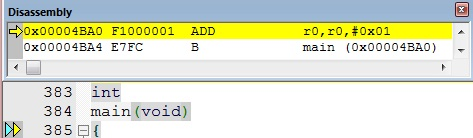
\includegraphics[scale=0.7]{ex2}
	\caption{The device executing the injected code. }\label{fig::ex}
\end{figure}


\begin{figure}[p]
	\centering
	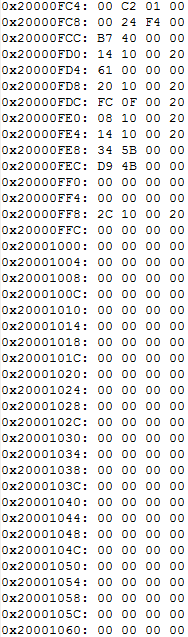
\includegraphics[scale=1]{StackBefore1}
	\caption{The stack prior to any tampering - 1. }\label{fig::st1}
\end{figure}
\begin{figure}[p]
	\centering
	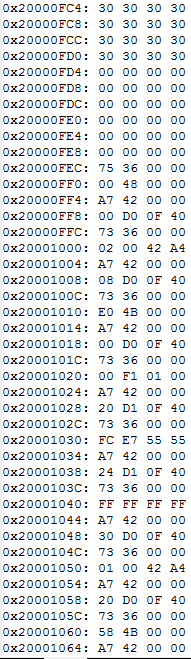
\includegraphics[scale=1]{stackAfter1}
	\caption{The stack after corruption - 1. }\label{fig::st2}
\end{figure}

\begin{figure}[p]
	\centering
	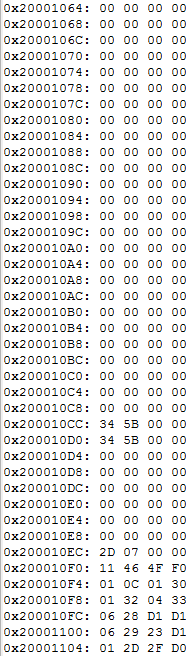
\includegraphics[scale=1]{StackBefore2}
	\caption{The stack prior to any tampering - 2. }\label{fig::st3}
\end{figure}
\begin{figure}[p]
	\centering
	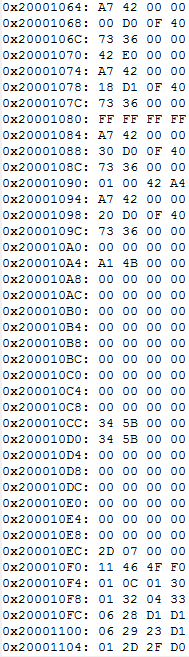
\includegraphics[scale=1]{stackAfter2}
	\caption{The stack after corruption - 2. }\label{fig::st4}
\end{figure}

\begin{figure}[p]
	\centering
	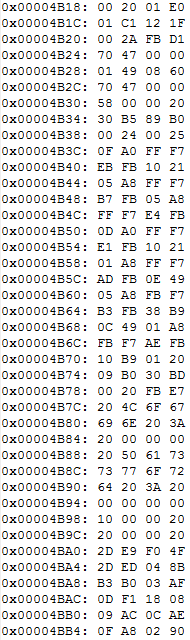
\includegraphics[scale=1]{FlashBefore.PNG}
	\caption{The flash memory at main prior to any tampering. }\label{fig::fl0}
\end{figure}
\begin{figure}[p]
	\centering
	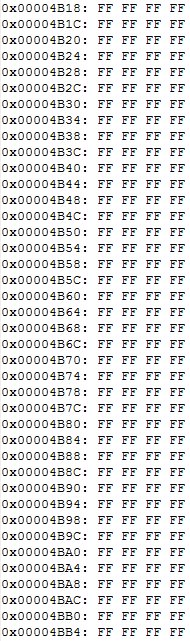
\includegraphics[scale=1]{FlashAfterErase}
	\caption{The flash memory after the erase of main(). }\label{fig::fl1}
\end{figure}

\begin{figure}[p]
	\centering
	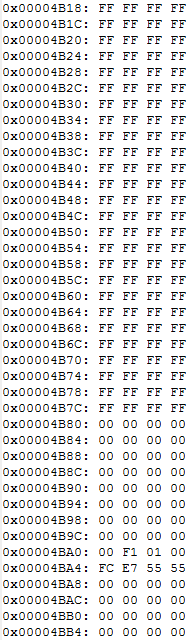
\includegraphics[scale=1]{FlashAfterWrite1}
	\caption{The flash memory after the write to main(). }\label{fig::fl2}
\end{figure}

\begin{figure}[p]
	\centering
	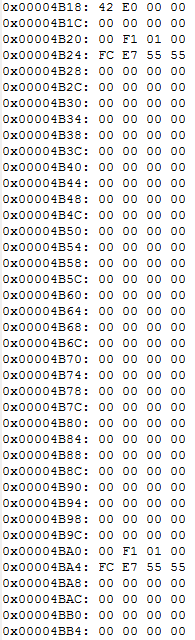
\includegraphics[scale=1]{FlashAfterWrite2}
	\caption{The flash memory after the write to the scatter function. }\label{fig::fl3}
\end{figure}
